% This is "sig-alternate.tex" V2.0 May 2012
% This file should be compiled with V2.5 of "sig-alternate.cls" May 2012
%
% This example file demonstrates the use of the 'sig-alternate.cls'
% V2.5 LaTeX2e document class file. It is for those submitting
% articles to ACM Conference Proceedings WHO DO NOT WISH TO
% STRICTLY ADHERE TO THE SIGS (PUBS-BOARD-ENDORSED) STYLE.
% The 'sig-alternate.cls' file will produce a similar-looking,
% albeit, 'tighter' paper resulting in, invariably, fewer pages.
%
% ----------------------------------------------------------------------------------------------------------------
% This .tex file (and associated .cls V2.5) produces:
%       1) The Permission Statement
%       2) The Conference (location) Info information
%       3) The Copyright Line with ACM data
%       4) NO page numbers
%
% as against the acm_proc_article-sp.cls file which
% DOES NOT produce 1) thru' 3) above.
%
% Using 'sig-alternate.cls' you have control, however, from within
% the source .tex file, over both the CopyrightYear
% (defaulted to 200X) and the ACM Copyright Data
% (defaulted to X-XXXXX-XX-X/XX/XX).
% e.g.
% \CopyrightYear{2007} will cause 2007 to appear in the copyright line.
% \crdata{0-12345-67-8/90/12} will cause 0-12345-67-8/90/12 to appear in the copyright line.
%
% ---------------------------------------------------------------------------------------------------------------
% This .tex source is an example which *does* use
% the .bib file (from which the .bbl file % is produced).
% REMEMBER HOWEVER: After having produced the .bbl file,
% and prior to final submission, you *NEED* to 'insert'
% your .bbl file into your source .tex file so as to provide
% ONE 'self-contained' source file.
%
% ================= IF YOU HAVE QUESTIONS =======================
% Questions regarding the SIGS styles, SIGS policies and
% procedures, Conferences etc. should be sent to
% Adrienne Griscti (griscti@acm.org)
%
% Technical questions _only_ to
% Gerald Murray (murray@hq.acm.org)
% ===============================================================
%
% For tracking purposes - this is V2.0 - May 2012

\documentclass{sig-alternate}
\usepackage{multirow}
\usepackage{graphicx}
\begin{document}

\title{Interactive Public Display}
\subtitle{- Mobile and Pervasive Computing}
%
% You need the command \numberofauthors to handle the 'placement
% and alignment' of the authors beneath the title.
%
% For aesthetic reasons, we recommend 'three authors at a time'
% i.e. three 'name/affiliation blocks' be placed beneath the title.
%
% NOTE: You are NOT restricted in how many 'rows' of
% "name/affiliations" may appear. We just ask that you restrict
% the number of 'columns' to three.
%
% Because of the available 'opening page real-estate'
% we ask you to refrain from putting more than six authors
% (two rows with three columns) beneath the article title.
% More than six makes the first-page appear very cluttered indeed.
%
% Use the \alignauthor commands to handle the names
% and affiliations for an 'aesthetic maximum' of six authors.
% Add names, affiliations, addresses for
% the seventh etc. author(s) as the argument for the
% \additionalauthors command.
% These 'additional authors' will be output/set for you
% without further effort on your part as the last section in
% the body of your article BEFORE s or any Appendices.

\numberofauthors{3} %  in this sample file, there are a *total*
% of EIGHT authors. SIX appear on the 'first-page' (for formatting
% reasons) and the remaining two appear in the \additionalauthors section.
%
\author{
% You can go ahead and credit any number of authors here,
% e.g. one 'row of three' or two rows (consisting of one row of three
% and a second row of one, two or three).
%
% The command \alignauthor (no curly braces needed) should
% precede each author name, affiliation/snail-mail address and
% e-mail address. Additionally, tag each line of
% affiliation/address with \affaddr, and tag the
% e-mail address with \email.
%
Geng Fu\thanks{This author will be graduating soon.}\\
	\affaddr{INI}\\
	\affaddr{Carnegie Mellon University}\\
	\email{gengf@andrew.cmu.edu }
\alignauthor
Vinay Kumar Vavili\thanks{This author will be graduating soon.}\\
	\affaddr{INI}\\
	\affaddr{Carnegie Mellon University}\\
	\email{vvavili@andrew.cmu.edu}
\alignauthor
Yalei Song\thanks{This author still has to ``suffer'' to lot.}\\
	\affaddr{ECE}\\
	\affaddr{Carnegie Mellon University}\\
	\email{yaleis@andrew.cmu.edu}
}

% Just remember to make sure that the TOTAL number of authors
% is the number that will appear on the first page PLUS the
% number that will appear in the \additionalauthors section.

\maketitle
\pagenumbering{arabic}

\section{Introduction}
Public displays are ubiquitous. They can be seen in many public locations including malls, schools, and coffee shops. Public displays share these characteristics:
\begin{itemize}
	\item They appear in public places (as mentioned above)
	\item Their locations are usually fixed (not portable)
	\item They are usually large in size
	\item People pass by or gather around the display
	\item There are limited interfaces. Keyboards, touch screens are usually not provided
	\item No internal memory available (it is just a screen)
\end{itemize}

With those characteristics, public displays are often being used as a screen to display content. It could be static content like posters, images and Ads; or it could be dynamics content like news channels, trends or music videos. However, public displays are not necessarily aware of its surroundings. Most importantly, displays don't respond to the presence of people. In other words, public displays are not interactive. For instance, a public display in a mall could show music videos of Justin Bieber all day long, even though none of the people in the mall is a Belieber\footnote{A huge fan of Justin Bieber.}.

\section{Objectives}
The objectives of this project are to make public displays interactive. We set different 
scenarios, such as cocktail parties where people mostly mingle with others; or a coffee 
shop where people stand in line waiting to order. Specifically, we hope to achieve two 
goals. First, we would like to encourage interaction between people and display, and 
also to make displays and people aware of each other's presence. Second, we would 
like to foster interaction between people and encourage discussion.

In order to engage people, we started with designing an application that attracts 
people's attention. Many ideas were emerged, such as developing games or tools that 
will allow people to participate in activities. We believe that game is an efficient way to 
gather people's attention in a short period of time, hopefully in a pleasant way also.

The objectives of the game are very simple. It allows people to interact with display and 
promote interaction between people quickly. Since we set up our game in scenarios like 
cocktail parties and coffee shops, where people are usually occupied, we want to make 
sure that players can join the game anytime. Moreover, players shall not feel obligated to stay in 
the game; she/he should be able to leave the game anytime. In additional, the game 
should not be too intellectual or difficult to play.

We conducted a series of brainstorming and came up with several game ideas, such as 
action game (e.g., darts, basketball), gambling game (e.g., roulette), word puzzle game 
and trivia game. We later realized that action requires too much commitment to the game 
and space for movement, which doesn't suit our scenarios; puzzle game involves too 
much intelligence and it is time consuming; whereas gambling game is basically random 
guess. As a result, developing trivia game(s) was a favorable idea.

\section{Game Ideas}
To ensure an abundant question pool for the trivia game, we utilized Google APIs which 
provide ample useful information.

\subsection{Battle of Cities}
Google radar search (part of Google Places API) provides number of a certain type of places 
(e.g., restaurant, bakery) in a given area. With this information we can develop a trivia game 
that is based on numbers of places in different cities. Here is a sample question: Which city 
has more bars, New York City or Shanghai?

We select more than 10 high-profile cities in both the eastern and western atmosphere and 
80 place types to generate questions.

\subsection{Translator's Dilemma}
Google translate game idea was emerged when browsing a website called 
Translation-telephone\cite{pamela:translation_telephone}, which is similar as the traditional ``Telephone'' game where people pass a message around a circle and see how it turns out at the end. In translation-telephone, a message gets translated to random languages and 
 back to the original language.

We thought it was an interesting idea and wanted to develop a game based on it. Google Translate is one of the most widely used translate engine, and it is a great tool to use in this game. In the same way as translation-telephone, we randomly select collections of languages and use Google translate API to generate translations. In addition, we have two collections (paths) of languages and provide one final translation. In the end, players will get to choose which path the final translation is generated from.

\section{Preliminary Design}
Our goal is to design games that are easy for user to understand; it should be straightforward and easy on the eye. To that end, we came up with a user interface prototype (Figure \ref{fig:pre_design}) that is to be used by both Battle of Cities and Translator's Dilemma. 

\begin{figure*}
	\centering
	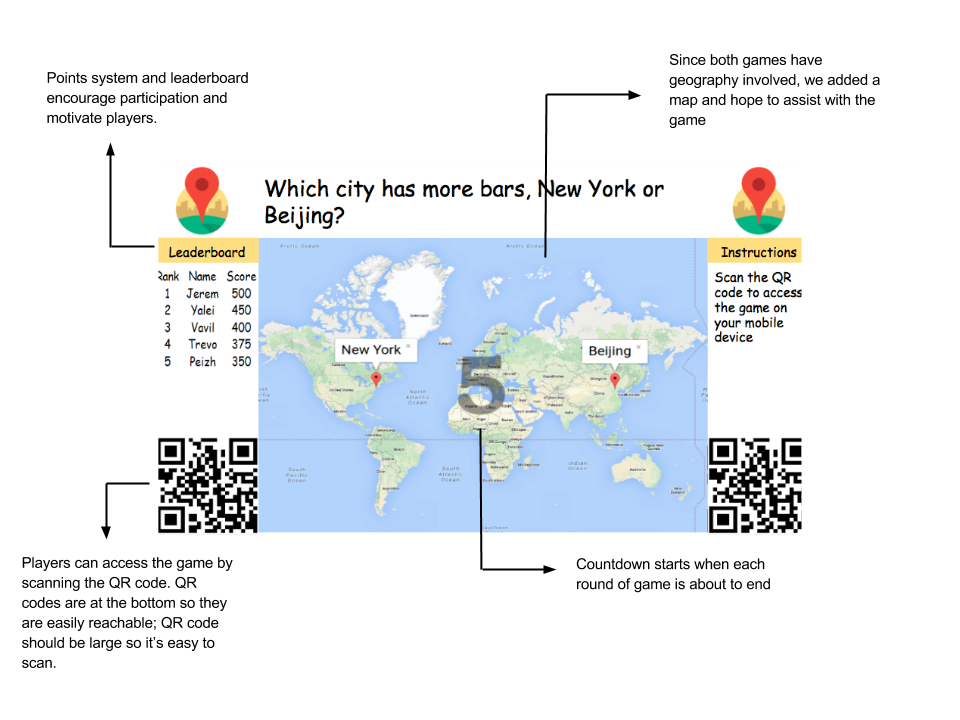
\includegraphics[width=0.8\textwidth,height=10cm]{preliminary_design.png}
	\caption{Preliminary Design}
	\label{fig:pre_design}
\end{figure*}

\section{User Study}
In order to evaluate the effectiveness of the games we developed and iterate the design, we conducted user studies. The user study was conducted in a student common on Carnegie Mellon University Silicon Valley campus. The students common is the hub of the building and there were hundreds of people passing by. We deployed here to attract more students to play and therefore obtain more feedback. The game was deployed on XX size Sharp display. A Macbook Pro was connected to the display to render the view in a web browser. A backend end server backed by Node.js, along with a CouchDB, was deployed at an EC2 instance on Amazon Web Service. The web page was loaded from the backend server to the web browser. Figure \ref{us:deployment} is a capture of the deployment. 

We invited some of students to play the game and there were some unsolicited involvement. After they played the game, we asked them to fill in a survey. The survey  focused on the game design, their behaviors in playing the game and their interaction among other players.

\begin{figure}
	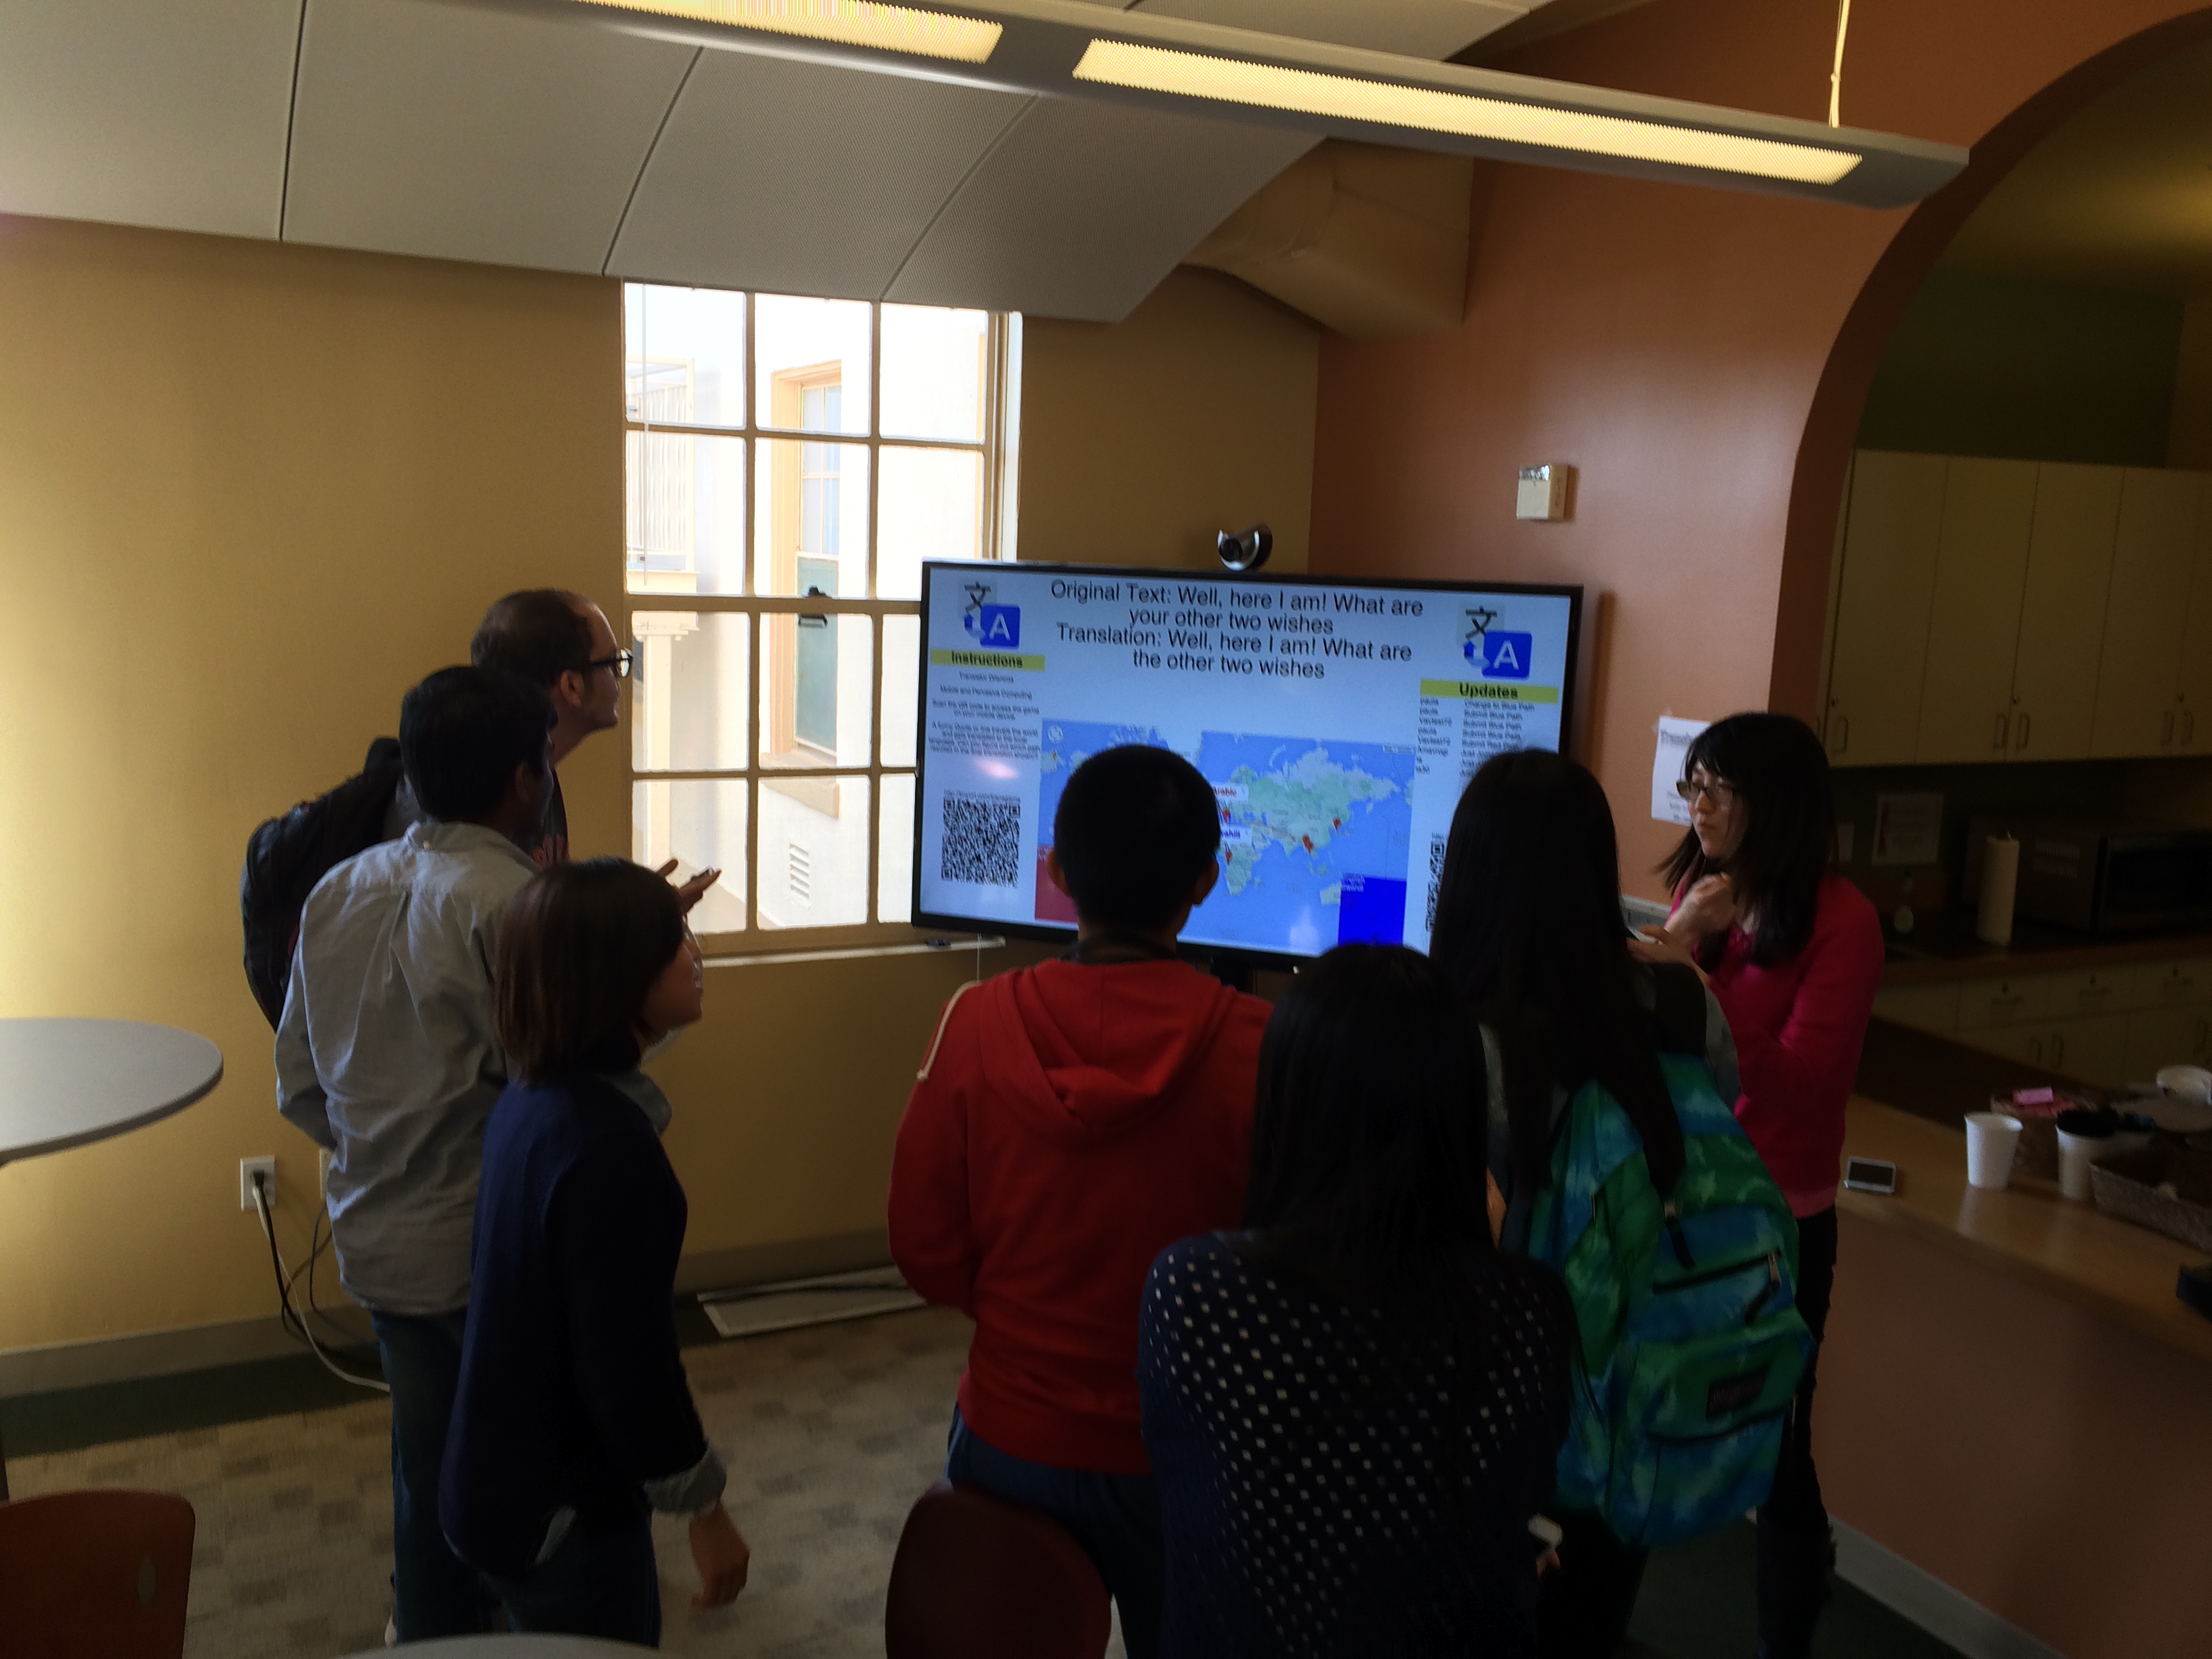
\includegraphics[width=\linewidth]{deploy.jpg}
	\caption{Deployment of Translator's Dilemma}
	\label{us:deployment}
\end{figure}

\section{Design Guidelines}
Table \ref{table:design_guidlines_summary} summarizes the design guidelines that we hope will assist the design of games for interactive public displays.

\begin{table*}[ht]
	%\captionsetup{justification=centering}
	\label{table:design_guidlines_summary}
	\begin{tabular*}{1\textwidth}{c | l}
 		\hline
		Aspect & Lesson\\ \hline
  		\multirow{4}{*}{Content} & The questions should be intuitive or easy to understand\\
 			& The answers should be correct or logical\\
 			& They are usually large in size\\
 			& People pass by or gather around the display\\ \hline
		\multirow{4}{*}{Player Perception} & Attention span of users is limited. The timing between rounds of games has to be reasonable
\\
 			& Make sure the player knows the status of the game at all times\\
 			& Players should be motivated\\ \hline	
	\end{tabular*}
	\caption{Design Guidelines Summary}
\end{table*}

The design guidelines were formulated based on user feedback and results from user studies conducted as part of the live deployment. We also used the results of user studies to evaluate whether we met the objectives of the game. The study responses were scaled from 1 to 10. We normalized the scaled responses to standard\cite{laerd:standard_score}. In simple terms, the percentage calculated from the z-score represents the percentage of responses that are greater than or equal to the benchmark selected during the z-score calculation. We have selected a benchmark of 8 for the scale from 1 to 10.

In the following subsections, we discuss each design guideline and the user study related to the guideline.

\subsection{The questions should be intuitive or easy to understand;\\
The answers should be correct or logical}

The first question we asked participants was, ``How easy is it for you to understand the objective of the game?''. 
Figure \ref{fig:p_easy_understand} shows the the responses for the game Battle of Cities and Figure \ref{fig:t_easy_understand} is the responses for Translator's Dilemma. 

\begin{figure}
	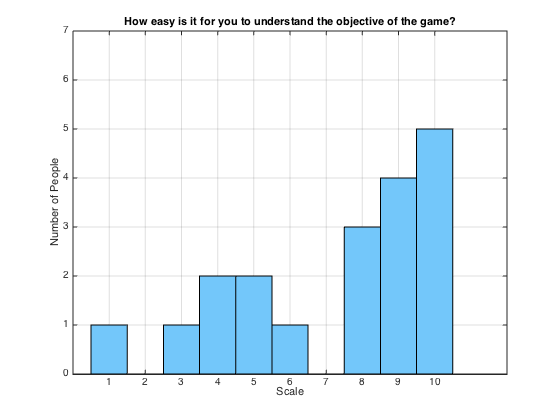
\includegraphics[width=\linewidth]{p_easy_understand.png}
	\caption{Battle of Cities - How easy is it for you to understand the objective of the game?}
	\label{fig:p_easy_understand}
\end{figure}

\begin{figure}
	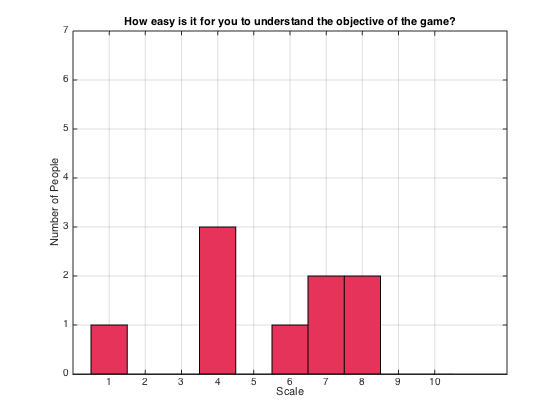
\includegraphics[width=\linewidth]{t_easy_understand.png}
	\caption{Translator's Dilemma - How easy is it for you to understand the objective of the game?}
	\label{fig:t_easy_understand}
\end{figure}

37.98\% of the participants felt that the Battle of Cities game was easy to understand. This was primarily because the question was quick to read and easy to understand. There was higher participation in the game as a consequence.

Compared to Battle of Cities, only 13.85\% of the participants felt that Translator's Dilemma game was easy to understand. As mentioned before, Translator's Dilemma game is based on the ``Telephone'' game. During the user study we noticed that it was very hard for participants to understand the objective of the game; most of them had not played the ``Telephone'' game before, or they could not relate Translator's Dilemma to the ``Telephone'' game. The question text was also long and complex in this case.

The following question we asked participants was, ``Did you discuss with others during the game?''. Figure \ref{fig:p_discuss} shows the the responses for the game Battle of Cities and Figure \ref{fig:t_discuss} is the responses for Translator's Dilemma.

\begin{figure}
	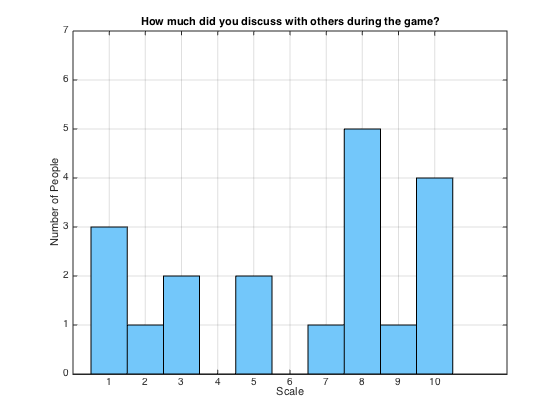
\includegraphics[width=\linewidth]{p_discuss.png}
	\caption{Battle of Cities - Did you discuss with others during the game?}
	\label{fig:p_discuss}
\end{figure}

\begin{figure}
	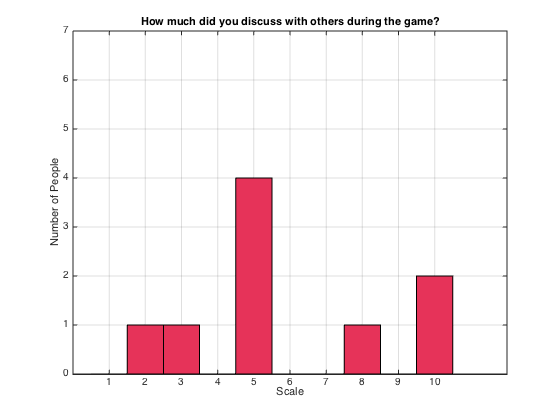
\includegraphics[width=\linewidth]{t_discuss.png}
	\caption{Translator's Dilemma - Did you discuss with others during the game?}
	\label{fig:t_discuss}
\end{figure}

27.30\% of participants discussed with others during the Battle of Cities game and 22.93\% of the participants discussed with others during Translator's Dilemma game. Knowledge of popular 
cities is common and there is enough time to discuss after deciding on the answer, therefore 
there is comparatively higher percentage of participants that discuss during the Battle of Cities Game. Whereas 
in Translator's Dilemma game, knowing all languages in the list is highly unlikely. 
The question is also long and complex so there is no time to discuss the results. 

During the user study we also noticed that all participants were surprised with answers that they thought were fairly obvious. The discrepancy happens as Google Radar search does not enough data to return answers that match user expectations. This causes participants to lose interest in the game. The above observations logically lead us to the following design decisions mentioned previously.

\subsection{Strike a balance between guess work and logical thinking}
We asked the participants, ``How did you choose your answer''. Scale 1 denotes completely random answer and 10 for logical answer. Figure \ref{fig:p_random_logical} shows the the responses for the game Battle of Cities and Figure \ref{fig:t_random_logical} is the responses for Translator's Dilemma. 

\begin{figure}
	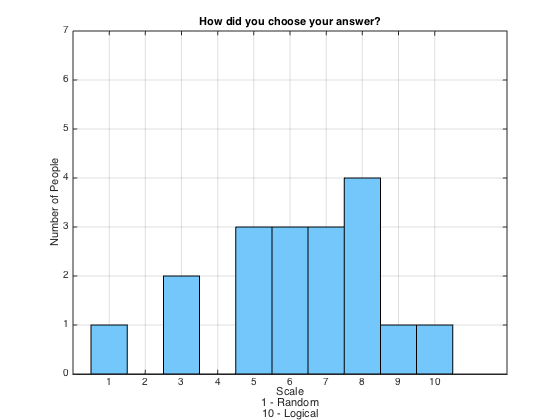
\includegraphics[width=\linewidth]{p_random_logical.png}
	\caption{Battle of Cities - How did you choose your answer?}
	\label{fig:p_random_logical}
\end{figure}

\begin{figure}
	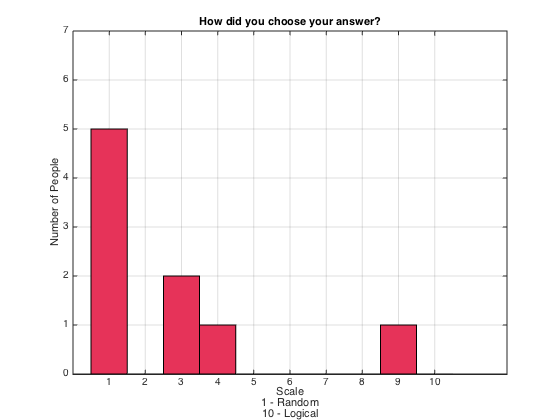
\includegraphics[width=\linewidth]{t_random_logical.png}
	\caption{Translator's Dilemma - How did you choose your answer?}
	\label{fig:t_random_logical}
\end{figure}

21.54\% of the participants in the Battle of Cities game felt that they chose the answer logically. This is mainly because the game itself has cultural and geographical hints that help users logically infer the number of places of a type in the given locations. 

Only 2.19\% of the participants of Translator's Dilemma game felt that they chose the answers logically. It is highly unlikely that a participant knows all languages that are in the question. The answer is also based on analyzing text rather than comparing numbers.

The above study leads us to believe that there should be a good mix of logical thinking and guess work to encourage interaction among participants. 

\subsection{Attention span of users is limited. The timing between rounds of games has to be reasonable}
During the course of the user study we observed that the timing between rounds in the game is a very important factor to keep participants engaged to the game. If the time is too long, participants get distracted from the game. If the time is too short, participants do not get time to interact with each other. 

The timing has to be adjusted based on the game too. There is no ``one size fits all'' solution. For instance, the time for the Translator's Dilemma game was 10 seconds more than that allotted for the Battle of Cities game due to the difficulty of the Translator's Dilemma game.

\subsection{Make sure the player knows the status of the game at all times}
We have a dynamic updates sidebar in the game that gets updated in real-time with messages about user activity including ``player joined'', ``player submitted answer'' and ``player changed answer''. We asked participants, ``Did you look at the updates sidebar?''. 68.42\% of the participants of Battle of Cities game and 77.77\% of the participants of Translator's Dilemma game noticed the updates. Both games have a high number which leads us to believe that it is an important feature for interactive displays.

\begin{figure}
	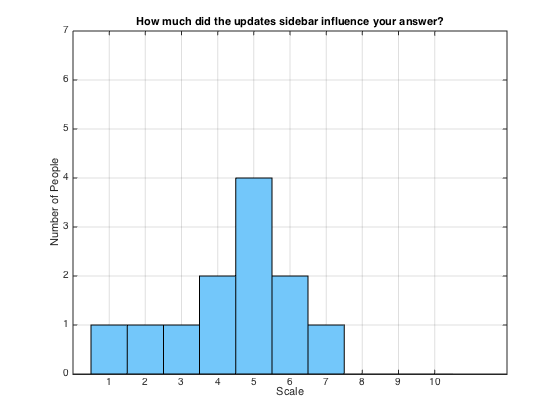
\includegraphics[width=\linewidth]{p_influence.png}
	\caption{Battle of Cities - How much did the updates sidebar influence your answer?}
	\label{fig:p_influence}
\end{figure}

\begin{figure}
	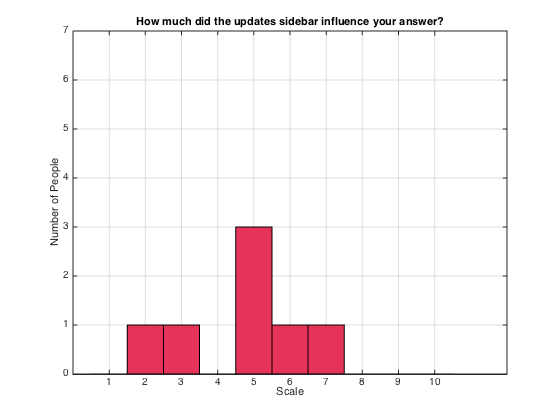
\includegraphics[width=\linewidth]{t_influence.png}
	\caption{Translator's Dilemma - How much did the updates sidebar influence your answer?}
	\label{fig:t_influence}
\end{figure}

The follow up question asked participants, ``How much did the updates sidebar influence your answer?''. Figure \ref{fig:p_influence} shows the the responses for the game Battle of Cities and Figure \ref{fig:t_influence} is the responses for Translator's Dilemma.

Surprisingly, only 1.47\% and 2.69\% of the participants in Battle of Cities and Translator's Dilemma game were influenced by the updates. This means that the updates bar primarily served as an activity monitor that provides feedback on user actions. The fact that a majority of the users noticed the updates but did not get influenced by it shows that it is very important to let the participant know the status of the game at all times.

In our prior design, we did not have a timer on the device that showed the time left in the current round. Lot of the participants were confused about what was happening after they selected their choice. The timer on the device helped alleviate this confusion.

\subsection{Players should be motivated}
We asked participants, ``Do you want to be on the leaderboard?''. Figure \ref{fig:p_leaderboard} shows the the responses for the game Battle of Cities and Figure \ref{fig:t_leaderboard} is the responses for Translator's Dilemma.

\begin{figure}
	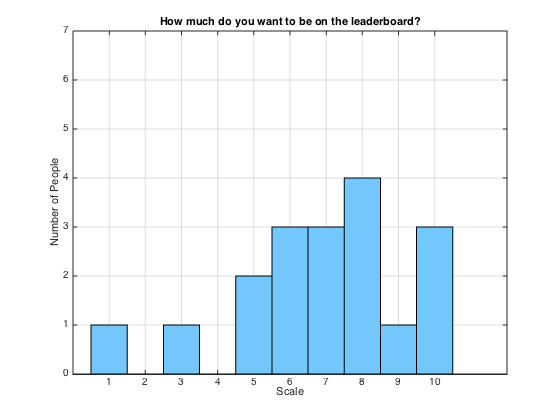
\includegraphics[width=\linewidth]{p_leaderboard.png}
	\caption{Battle of Cities - Do you want to be on the leaderboard?}
	\label{fig:p_leaderboard}
\end{figure}

\begin{figure}
	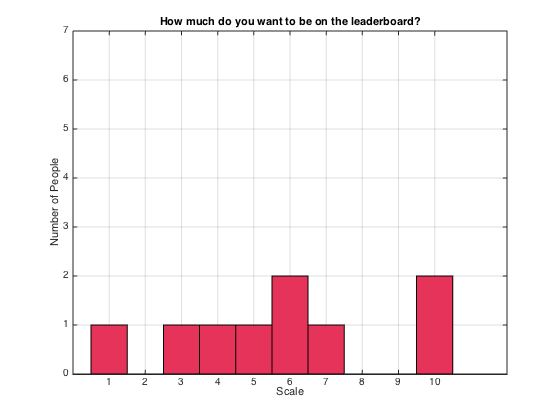
\includegraphics[width=\linewidth]{t_leaderboard.png}
	\caption{Translator's Dilemma - Do you want to be on the leaderboard?}
	\label{fig:t_leaderboard}
\end{figure}

28.53\% and 22.8\% of the participants from the Battle of Cities and Translator's Dilemma game want to be on the leaderboard respectively. Battle of Cities has comparatively higher number as the game itself is easier and leads to more participation. The difficulty of the Translator's Dilemma game discouraged participation and there was no incentive to be on the leaderboard. This observation leads us to believe that participants should be motivated to participate. Points system and leaderboard encourage participation and motivate players.

\section{Lessons}

We set up an approximately one-month-long deployment in a common area on campus where many students pass by.
Deployment was an essential part of our project, and we learned valuable lessons.
In this section, we discuss lessons learned in detail.

\subsection{Do not underestimate the efforts to implement web page on mobile devices}
The challenge of making a fluid UI is to deal with different resolutions of 
screens. A basic solution is using relative units such as em or percentage(\%) 
instead of pixels(px). However, in deployment we found out that since the 
dimensions of screens are different, the UI is not consistent across 
all screens. To handle the problem of different screens' dimensions we used 
viewport, which arranges elements by the actual size of the screen. Users 
may hold the device in different orientations too. We used CSS media query 
to detect the orientation of the devices and then display the elements on
 the screen. Even though we spent a lot efforts on device UI, the UI is not 
 consistent on old devices.
 
\subsection{Public display should be self-configurable}
Initially, the URL of the backend 
server was hard-coded to ensure users can connect to backend servers, and QR code was static. Consequently, when the backend server is 
deployed in another location, all those static components need to be configured 
before deployment. A solution to ease deployment is to ensure 
that web browser is aware of where the page is loaded from.

\subsection{Long-duration deployment discloses bugs}
Many potential bug weren't revealed until 
long-duration deployment. During deployment, problems may arise from 
unreliable dependencies, race conditions between multiple players operating 
at the same time and so on.

\subsection{Fault-tolerance at public display}
In the deployment, we often don't have
direct control of the public display. Display may lose connection to
the server, in which situation the public display should be able to reconnect to 
backend server. If bugs are found in the frontend page, the display needs to 
reload the web page. A script which periodically reloads the web page is helpful 
in deployment.

\subsection{Backend server should be publicly addressable}
A common mistake in 
deployment is to deploy the backend server with a private IP address. Due to 
the NAT problem, only the devices that are in the same network can access the 
game. Therefore, having a public addressable interface is essential to the backend server.

\subsection{Provide alternative way to allow players to access the game}
In the deployment, we assumed 
that users will scan the QR code to access the game. It turned out that most of devices 
were not equipped with QR code scanner, and players are reluctant to install one. 
Alternative ways such as tiny URL is helpful. 

\subsection{Carefully choose the place to conduct user study}
The place of our deployment was in 
a student common area. Students mostly were in a rush. Hence, unsolicited involvement 
was low. Since our games are designed for public locations (e.g., cocktail parties, coffee shops) and we need to measure the interaction among players; in order to conduct user studies effectively, we need a large group of players to play the game simultaneously.

\section{Conclusions}


\section{Future Work}


\bibliographystyle{plain}
\bibliography{sigproc}

\end{document}
